%!TEX root = ../Thesis.tex
\section{Dokumentation der Software}

\subsection{Dokumentation der Paketstruktur des Android-Projektes [Falk]}

Die Applikation liegt im Paket \code{de.fhdw.wip.rpntilecalculator} vor und ist mit verschiedenen Klassen realisiert, welche in eine Paketstruktur eingebettet sind. Diese Paketstruktur orientiert sich an dem gewählten UI Design Pattern MVP. 

Eines dieser Pakete trägt den Namen \code{Model}. Dieses ist in vier weitere Unterpakete unterteilt, welche den verschiedenen Schemen nachempfunden sind sowie einen für den Stack. In diesen Unterpaketen befinden sich verschiedene Klassen, die zusammen das Model bilden. 

Das \code{View}-Paket besteht ebenfalls aus mehreren Unterpaketen. Dort findet man zum einen die \code{MainActivity}, welche die Hauptaktivität der Applikation darstellt. Darüber hinaus befinden sich dort die Schemen und Util-Klassen der Kacheln. Es gibt noch die drei Pakete \code{Layout}, \code{Menu} und \code{Schemes}. In \code{Layout} befinden sich Funktionen zum Darstellen, Speichern und Laden der Kacheln. In \code{Schemes} befinden sich Vorlagen für Tiles und in \code{Menu} sind sämtliche Menüs gespeichert. 

Im \code{Presenter}-Paket befindet sich lediglich der Presenter. Dieser wird verwendet, um die Einzelteile des \code{View}- und \code{View}-Pakets zu verbinden. 

\begin{figure}[!h]
	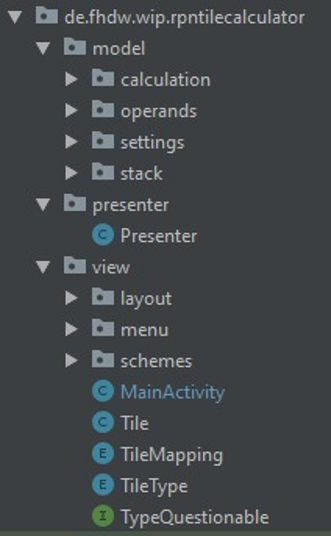
\includegraphics[scale=1]{img/ordnerstruktur}
	\caption[Ordnerstruktur]{Ordnerstruktur\footnotemark}
\end{figure}
\footnotetext{eigene Darstellung (Screenshot aus Android Studio)}

\begin{figure}[!h]
	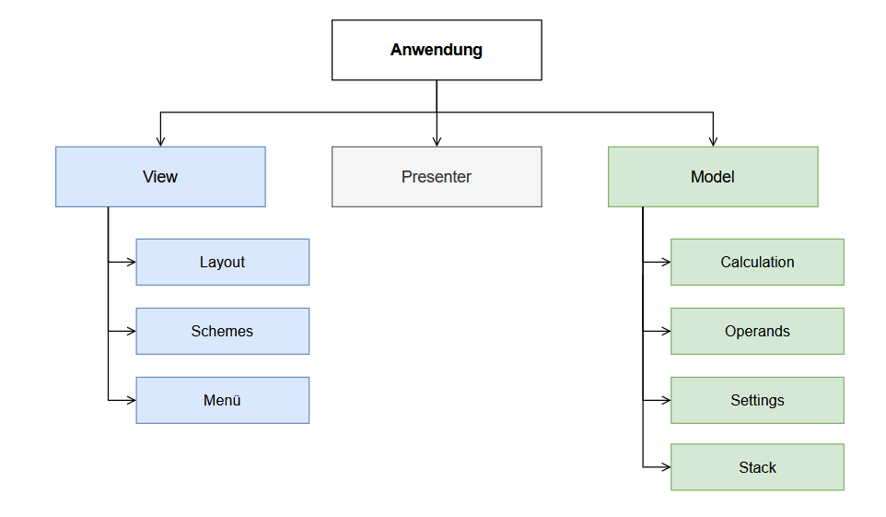
\includegraphics[scale=1]{img/ordnerstruktur2}
	\caption[Ordnerstruktur Schema]{Ordnerstruktur Schema\footnotemark}
\end{figure}
\footnotetext{eigene Darstellung}

\subsection{Dokumentation der View}

In den folgenden Kapiteln wird die Implementierung des Frontends der Applikation, der sogenannten View, und jeglichen zugehörigen Implementierungen, dargestellt.

\subsubsection{Activities [Bockhorn]}

Die Applikation wird durch den Aufruf der sogenannten \code{MainActivity} vom Android System beim Öffnen der Anwendung gestartet. Da die Menüführung nicht auf Activities basiert und jegliche Layouts dynamisch geladen werden, bleibt die \code{MainActivity} die einzige Activity der Applikation

Im MVP Pattern ist die \code{Activity} der View zugeordnet. Sie lädt unter anderem vertikale und horizontale Layouts vor und stellt eine Methode zur Darstellung dieser bereit. Auch wird ein Listener erstellt, der nach Änderungen der Bildschirmausrichtung horcht und passende Layouts lädt.

\paragraph{Klasse: MainActivity}

\textbf{Beschreibung:} Activity, die beim Starten der Anwendung aufgerufen wird und das Layout \code{activity\_main.xml} aufruft. Dieses Layout ist jedoch leer, da alle Inhalte dynamisch geladen werden. Es lädt auch Taschenrechner-Layouts vor und stellt Methoden zur Darstellung dieser bereit.

Die \textbf{Methode} \code{onCreate()} lädt die Layouts vor, erstellt einen \code{Listener}, der überwacht ob sich die Orientierung verändert und öffnet daraufhin das erste Layout.

\textbf{Methode} \code{setTileLayout()} lädt ein Layout in die View.

\subsubsection{Generische Kachelgestaltung [Bockhorn]}

Die generische Gestaltung der Kacheln wurde gemäß dem Entwurf so umgesetzt, dass eine Trennung zwischen Kacheln, die als Buttons vom Kontext der Applikation abhängig sind, und Kacheln, die vom Kontext unabhängig sind, ermöglicht wird. Dies dient unter anderem dem Vorladen von Layouts zur Optimierung der Ladeperformance. Außerdem wird so die Definition des Kacheltypen und dessen spezialisierte Inhalte auf die vom Kontext unabhängigen Kachelschemata (\code{TileSchemes}) ausgelagert. 

Als logische Abtrennung kann man sich merken, dass Kacheln (\code{Tiles}) lediglich für die Kommunikation mit dem Nutzer zuständig sind, während die \code{TileSchemes} die restliche Frontend-Logik beinhalten.

\subsubsection{Kontextbezogene Kacheln [Bockhorn]}

Die Tiles werden mit Bezug auf den Kontext, also die aktuell dargestellte Activity, erstellt. Sie dienen als generische Kachelklasse, dessen Funktionalitäten unabhängig vom Kacheltypen gebraucht werden.

Ein Tile, als Unterklasse des \code{AppCompatButton} von Android, entwirft beim Anklicken ein Event, welches von registrierten \code{OnClickListenern} abgefangen werden kann. Für die einzelnen Tiles wird der \code{Presenter} als \code{OnClickListener} registriert, sodass dieser die vom Nutzer getätigten Klicke verarbeiten kann. Zusätzlich wird dem \code{Tile} als \code{OnLongClickListener} das Menü \code{TileTypeInput} übergeben, welches bei langem Klicken geöffnet wird und somit die Bearbeitung des Kacheltypen ermöglicht.

\begin{figure}[!h]
	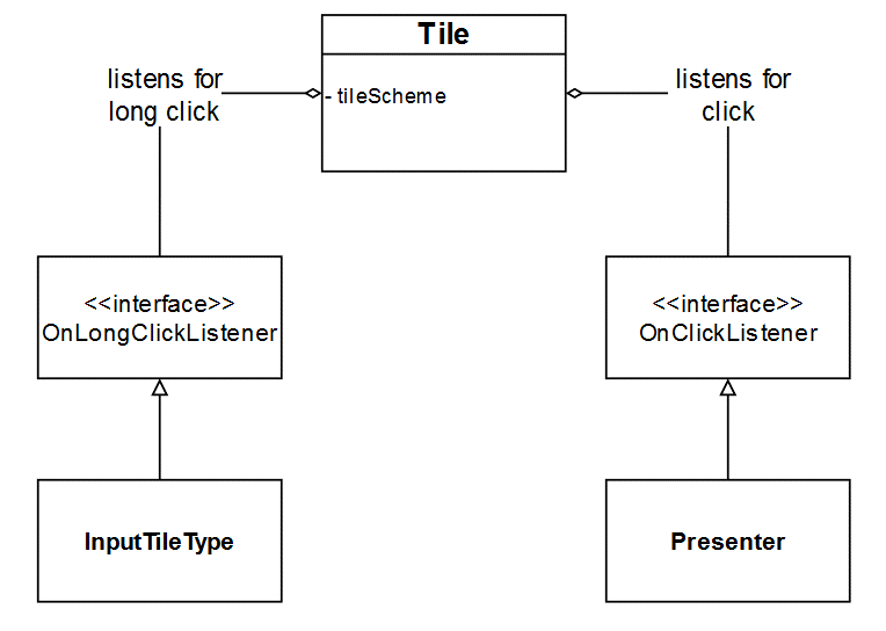
\includegraphics[scale=1]{img/listener-von-tile}
	\caption[Listener von Tile]{Listener von Tile\footnotemark}
\end{figure}
\footnotetext{eigene Darstellung}

Die Informationen über den Kacheltypen des \code{Tiles} befindet sich im \code{TileScheme} des \code{Tiles}. Werden nun die Inhalte, oder gar der Kacheltyp des \code{Tiles} verändert, so wird das Aussehen des \code{Tiles} anhand des aktuellen \code{TileSchemes} aktualisiert. Ähnlich stellt ein \code{Tile} verschiedene Animationen bereit, die zum Beispiel beim Laden oder Speichern des \code{Tiles} aufgerufen und abgespielt werden können.

\paragraph{Tile [Bockhorn]}

\textbf{Superklasse:} \code{AppCompatButton}

\textbf{Beschreibung:} Agiert als Button auf einem Kontext, dessen Inhalt und Typ durch ein \code{TileScheme} definiert sind. Einfaches Klicken wird vom \code{Presenter} abgefangen und gedrückt halten öffnet ein Auswahlmenü für die Kachelart. 

\textbf{Methode} \code{update} Aktualisiert das \code{Tile} mithilfe eines neuen \code{Schemes}. Setzt dabei Hintergrund Ressource und Text

\textbf{Methode} \code{enableMenulistener} Aktiviert die Menüfunktion für dieses \code{Tile}

\subsubsection{Kontextfremde Kacheln [Gentges]}

Die \code{TileSchemes} stehen in keiner Beziehung zum Kontext der Anwendung. Dennoch wird in ihnen der Text und das Design des letztendlichen \code{Tiles} gespeichert. Im Gegensatz zu den \code{Tiles} differenzieren \code{TileSchemes} hier zwischen Kachelarten. Die Grundeigenschaften eines \code{TileSchemes}, also die Information darüber um welche Art von Kachel es sich handelt, und was genau der Inhalt ist, werden in der Superklasse \code{TileScheme} definiert. Ersteres liegt in Form eines sogenannten \code{TileMappings} vor. Für jede der bestehenden Kachelarten wurde eine Unterklasse implementiert, welche die Eigenschaften von \code{TileScheme} erbt und weitere artbezogene Inhalte definiert. In Kombination mit einem \code{Tile} können so andere Komponenten der Applikation, wie beispielsweise der \code{Presenter}, die Kachelart des \code{TileScheme} erfragen und den vorliegenden Inhalt für die auszuführenden Prozesse extrahieren.

\begin{itemize}
	\item Das \code{ActionTileScheme} ist die Implementierung eines \code{TileScheme} vom Typ Action, (auch \code{Operator}) der Inhalt und Typ um eine instanziierte Action erweitert. Dank der ähnlich polymorphen Struktur der \code{Action}s, kann so mit einem simplen Methodenaufruf jede Form von \code{Action}, die im Schema hinterlegt ist, angesprochen und ausgeführt werden.
	\item Ein \code{SettingTileScheme} erbt ebenfalls von \code{TileScheme}, aber liefert zusätzlich Informationen über ein sogenanntes \code{Setting}, welches ähnlich wie eine \code{Action} über eine vererbte Methode anzusprechen ist.
	\item Ein \code{OperandTileScheme} ist gleich aufgebaut, beinhaltet aber Operanden, die als Grundlage für die Kalkulation mit \code{Action}s dienen.
	\item Das Klicken auf ein \code{Tile} des Stacks wird intern gleich gehandhabt, wie das Klicken eines Operanden. Jedoch besitzen Tiles aus dem Stack eine Reihenfolge, die im \code{StackTileScheme} als Rang hinterlegt wird. Um die gleiche Behandlung eines potenziellen Operanden im Stack zu gewährleisten, erbt \code{StackTileScheme} nicht von \code{TileScheme}, sondern von \code{OperandTileScheme}. 
	\item Ein \code{HistoryStackTile} ist ebenfalls so aufgebaut, wie ein \code{StackTileScheme}, und erbt daher dessen \code{Attribute}.
\end{itemize}

Die Erstellung einzelner \code{TileSchemes} erfolgt mithilfe des Factory-Method-Design-Pattern. Hierzu stellt die abtrakte Superklasse \code{TileScheme} zwei Methoden zur Verfügung. Innerhalb dieser Methoden wird anhand des \code{TileMappings} zwischen den verschiedenen Kachelarten differenziert und der passende Konstruktor der Unterklasse aufgerufen. In einer Methode erfolgt die Erstellung des \code{TileScheme} Inhalts durch die Einlese einer Zeichenkette. Dies findet beispielsweise bei der Kreierung von \code{TileSchemes} oder nach der Auslese eines im internen Speicher gespeicherten Layouts, Anwendung. Als zweite Option kann aus einem bereits bestehenden Operanden ein \code{TileScheme} der Art Operand, Stack oder Historie erstellt werden. Dadurch, dass Stack und Historie eines Layouts regelmäßig aktualisiert werden müssen, bietet sich die performante Erstellung von \code{TileSchemes} mithilfe bestehender Operanden, gegenüber der aufwendigen erneuten Auslese aus einem String, an.

Im Kontrast zu den Tiles, die eine Methode zum Aktualisieren der Inhalte bereitstellen, müssen \code{TileSchemes} mithilfe der genannten Methoden rekreiert werden. Kann eine Kachelart nicht identifiziert werden, oder sind die Angaben über den Inhalt der Kachel unkorrekt, so wird ein \code{ErrorTileScheme} erstellt, das visuell von jeder anderen Art zu unterscheiden ist und den Entwicklern somit über den Fehler Bescheid gibt.

\paragraph{Abstrakte Klasse: TileScheme}

\textbf{Beschreibung: }Abstrakte Superklasse, die neben den artübergreifenden Inhalten der \code{TileSchemes}, Methoden zur Kreierung dieser gemäß des Factory-Method-Design-Pattern bereitstellt.

\textbf{Methode} \code{createTileScheme()} liefert in Abhängigkeit vom angegebenen \code{TileMapping} eine Instanz einer Unterklasse des \code{TileSchemes}. Die Erstellung von \code{TileSchemes} für \code{Actions} und \code{Settings} ist lediglich durch die Eingabe von Zeichenketten möglich. \code{TileSchemes} der Arten \code{Operanden}, \code{Stack} und \code{Historie} können zusätzlich aus bestehenden \code{Operanden} erstellt werden. 

\paragraph{Klasse: ActionTileScheme}

\textbf{Superklasse:} \code{TileScheme}

\textbf{Beschreibung:}\code{TileScheme} für Operatoren. \code{Action}, die ausgeführt werden soll, als Zusatzinformation. Inhalt ist der Text der Kachel.

\paragraph{Klasse: SettingTileScheme}

\textbf{Superklasse:} \code{TileScheme}

\textbf{Beschreibung:} \code{TileScheme} für Einstellungen. \code{Settings}, die ausgeführt werden soll, als Zusatzinformation. Inhalt ist der Text der Kachel. 

\paragraph{Klasse: OperandTileScheme}

\textbf{Superklasse:} \code{TileScheme}

\code{Beschreibung:} \code{TileScheme} für Operanden. Bei der Erstellung aus Text wird der String mithilfe \textit{Reflections} zu einem Operanden übersetzt.

\paragraph{Klasse: StackTileScheme}

\textbf{Superklasse:}\code{OperandTileScheme}

\textbf{Beschreibung:}\code{TileScheme} für Operanden im Stack. Wird genauso behandelt wie ein \code{OperandTileScheme}, doch verfügt zusätzlich über eine Information über den Rang der Kachel im gesamten Stack.

\paragraph{Klasse: StackTileScheme}

\textbf{Superklasse:} \code{OperandTileScheme}

\textbf{Beschreibung:} \code{TileScheme} für Operanden im Stack. Wird genauso behandelt wie ein \code{OperandTileScheme}, doch verfügt zusätzlich über eine Information über den Rang der Kachel im gesamten Stack.

\paragraph{Klasse: HistoryTileScheme}

\textbf{Superklasse:} \code{StackTileScheme}

\textbf{Beschreibung: }\code{TileScheme} für Operanden in der Historie. Wird genauso behandelt wie ein \code{OperandTileScheme}, doch verfügt zusätzlich über eine Information über den Rang der Kachel im Gesamtstack.

\paragraph{Klasse: ErrorTileScheme}

\textbf{Superklasse:} \code{TileScheme}

\textbf{Beschreibung: }\code{TileScheme} für die Ausnahmesituation, dass ein reguläres \code{TileScheme} nicht geladen werden konnte

\subsubsection{Kacheltypdefinition durch Enumartion [Pham]}

Wie zuvor erläutert, erstellt die Klasse \code{TileSchemes} ein passendes Schema anhand eines sogenannten \code{TileMappings}. Ein \code{TileMapping} ist im Endeffekt eine konkrete Definition einer Kachel im Frontend-System. Hierzu beinhaltet das entsprechende \code{TileMapping} jegliche Informationen, die für eine bestimmte Kachel von Relevanz sind. 

Durch die Deklaration als Enum werden diese Informationen mit einer Zeichenkette zur Einlese in Verbindung gebracht. 

Für den Operator \code{-} (\code{Minus}) ist dies beispielsweise die Kachelart (\code{Action} / \code{Operator}), eine Referenz auf die passende \code{Action} Klasse und den Anzeigetext der Kachel \code{-}, die mit dem Text \code{A\_MINUS} betitelt werden. 

Die einzelnen Definitionen liegen in Form einer Java-Enumeration vor. Ein Beispiel für eine solche Definition sieht wie folgt aus:

\code{A\_MINUS(TileType.ACTION, Minus.getInstance(), "-")}

Neben Operatoren werden im Enum die anderen Datentypen ebenfalls angelegt. Technisch wurde dies durch die Verwendung von überladenen Konstruktoren ermöglicht und die \code{TileSchemes} wissen, welche Informationen gebraucht werden. Zur Definition der Kachelart selbst wurde eine weitere Enumeration mit folgenden Werten angelegt:

\begin{itemize}
	\item \code{Stack}
	\item \code{History}
	\item \code{Operand}
	\item \code{Action}
	\item \code{Setting}
	\item \code{Error}
\end{itemize}

Zu den Kachelarten sind Design-Ressourcen hinterlegt, welche die Gestaltung der Kacheln je nach Typ definiert.

\paragraph{Enumeration: TileMapping}

\textbf{Beschreibung: }Definiert Kacheln und dessen wichtigste Elemente. Wird außerdem zur Einlese von Texten genutzt.

\textbf{Bsp:} \code{A\_MINUS(TileType.Action, Minus.getInstance(), '' -'')}

\paragraph{Enumeration: TileType}

\textbf{Beschreibung: }Definiert die verschiedenen Kachelarten und ihre Design Ressourcen

\textbf{Bsp:} \code{ACTION(R.drawable.tile \_operator \_blue)}

\subsubsection{Gruppierung der Kacheln im Layout Container [Bockhorn]}
Gemäß dem Entwurf werden die Kacheln, sowohl \code{Tiles} als auch \code{TileSchemes}, in einem einheitlichen Container gespeichert. Das sogenannte \code{TileLayout} beinhaltet und bietet so dem Presenter eine zentralisierte Stelle zur Kommunikation mit Kacheln.

Insgesamt werden drei Bereiche unterstützt:
\begin{enumerate}
	\item Das Laden von kontextfremden \code{TileSchemes} in kontextbezogene \code{Tiles}. Grundsätzlich ist das \code{TileLayout} zwar unabhängig vom Applikationskontext, kann jedoch per Methode eine View für einen Kontext erstellen. Die Übersetzung erfolgt mit einer Darstellung in einer sogenannten \code{TableView} von Android. Neben der zweidimensionalen Liste an \code{Tiles} werden Listen für Stack und Historie geführt, die dann getrennt adressierbar sind.
	\item Die Aktualisierung von \code{Tiles} bei Änderungen im Stack, der Historie oder Anpassungen des Layouts. Hierbei ist zu erwähnen, dass nie das gesamte Layout aktualisiert wird, sondern nur Stack oder Historie. Beide werden mithilfe der korrespondierenden Listen im Presenter verglichen und aufgefüllt. Die Aktualisierung eines \code{Tiles} erfolgt durch die Kreierung eines neuen \code{TileSchemes}.
	\item Das Speichern des aktuellen \code{TileLayouts} durch die Zurückübersetzung von kontextbezogenen \code{Tiles} in kontextfremde \code{TileSchemes} zur Weiterverarbeitung durch den sogenannten \code{TileLayoutLoader}.
\end{enumerate}
Das \code{TileLayout} selbst wird mithilfe der \code{TileLayoutFactory} unter Verwendung des Factory-Design-Patterns aus einer Zeichenkette geladen. Das persistente Speichern und Laden dieser Zeichenkette und der Bezeichnung des \code{TileLayouts} selbst wird vom \code{TileLayoutLoader} orchestriert (siehe Kapitel~\ref{subsection:dokumentation-der-persistenten-datenhaltung}).

\para{Klasse: TileLayout}
\textbf{Methode} \code{createView} erstellt eine zweidimensionale Liste an \code{Tiles} aus der zweidimensionalen Liste an \code{TileSchemes}. Währenddessen werden eine \code{TableView} zusammengebaut und zurückgegeben und den eigenen Stack und die Historie Listen gesetzt.

\textbf{Methode} \code{pushStack2Presenter} übergibt dem Presenter den aktuellen Stack, z.B. zum Laden der Anwendung

\textbf{Methode} \code{pushHistoryStack2Presenter} übergibt den aktuellen History Stack, z.B. zum Laden der Anwendung

\textbf{Methode} \code{updateStack} aktualisiert jegliche \code{Tiles} im Stack durch den im Presenter geführten Stack an Operanden

\textbf{Methode} \code{updateHistoryStack} aktualisiert jegliche \code{Tiles} im History Stack durch die im Presenter geführte Historie

\textbf{Methode} \code{generateLayoutText} Generiert eine Zeichenkette im CSV-Format anhand der zweidimensionalen Liste an \code{Tiles}

\para{TileLayoutFactory}
\textbf{Beschreibung}: Factory für \code{TileLayouts}, die anhand einer Zeichenkette ein passendes Layout erstellt

\textbf{Methode} \code{createView} erstellt eine zweidimensionale Liste an \code{Tiles} aus der zweidimensionalen Liste an \code{TileSchemes}. Währenddessen werden eine \code{TableView} zusammengebaut und zurückgegeben und den eigenen Stack und die Historie-Listen gesetzt.

\subsubsection{Implementierung der Menüsteuerung [Istogu]}

In diesem Abschnitt wird die Umsetzung der Planung für die Menüsteuerung aufgegriffen. Als erstes wird die Architektur des Quellcodes näher dargelegt. Darauf anschließend wird sich mit der Implementierung der Zwischenmenüs und der Eingabeansicht für eine Auswahl an Operanden befasst.

\paragraph{Klasse: Dialogmenu [Istogu]}

Bei der \code{DialogMenu} handelt es sich um eine abstrakte Klasse, das von \code{View.OnClickListener} implementiert wird. Der Konstruktor erwartet folgende Parameter:  

\begin{itemize}
	\item \code{MainActivity context}
	\item \code{Tile displayTile}
	\item \code{DialogMenu last}
\end{itemize}

In dem Konstruktor wird ein \code{Dialog}-Objekt erstellt. Dabei werden initial bestimmte Attribute für das \code{Dialog} festgelegt, die für alle nachfolgenden Menüs gelten sollen. Als Beispiel kann hier aufgeführt werden, dass der Titel festgelegt wird. Zudem wird bestimmt, dass das Fenster zentral erscheint. Dieser Dialog wird erst angezeigt, wenn der \code{OnClickListener} ein Click vom vorherigen Dialog registriert. Zusätzlich wird \code{ContentViewID} über die Methode \code{setContentView()} festgelegt, die auf die einzelne \code{xml}-Dateien referenzieren. 

Die Methode \code{dismissAll()} sorgt dafür, dass beim Verlassen des Dialoges alle vorherigen Dialoge mitgeschlossen werden. Durch die Umsetzung des Schließens der vorherigen Dialoge erfolgt das rekursive Aufrufen der Methode \code{dismissAll()} von dem höheren gestellten Dialog-Objekt. Daher wird eine Referenz zu dem letzten Dialog benötigt. Der erste Dialog erhält ein \code{null}-Objekt, das bei der \code{dismissAll} überprüft wird.   

Grundsätzlich werden Dialoge geschlossen, wenn der Nutzer außerhalb des Dialoges mit der Benutzeroberfläche reagiert oder über den Quellcode \code{dialog.dismiss()} aufgerufen wird.  

\paragraph{Klasse: InputTileType [Istogu]}

Die Klasse erbt von der abstrakte Klasse \code{DialogMenu} und verweist über den \code{contentView} auf die \code{xml}-Datei. Dabei werden die Layouts (\code{xml}) mithilfe der Klasse \code{R.java} verbunden. Diese Klasse wird während des Kompilierens Referenzen zu den Ressourcen der Applikation erstellt. 

Zu den Ressourcen zählen unteranderem Bilder, \code{XML}-Ansichten und deren Komponenten wie Buttons. Die Referenzen zu den Buttons werden danach verwendet, um auf die Objekte über die Methode \code{dialog.findViewById()} zuzugreifen. In dem Konstruktor werden zu den jeweiligen Buttons ein \code{OnClickListener} festgesetzt, der ein neues Objekt vom Typ \code{InputTileMapping} erzeugt.

\paragraph{Klasse: InputTileMapping [Pham]}
Die Klasse \code{InputTileMapping} erbt ebenfalls vom \code{DialogMenu} und dient der Eingabe von konkreten, in \code{TileMapping} definierten, Kacheln. Durch die generische Implementierung und dynamische Befüllung des Menüs wird dem Nutzer eine einheitliche Eingabefunktionalität für unterschiedliche Kacheltypen ermöglicht. 

\begin{figure}[h]
	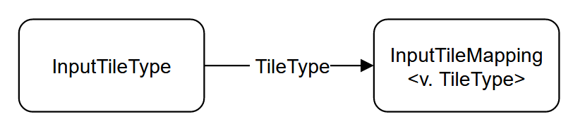
\includegraphics[scale=1]{img/relation-tiletype-tilemapping}
	\caption[Relation zwischen InputTileType und InputTileMapping]{Relation zwischen InputTileType und InputTileMapping\footnotemark}
\end{figure}
\footnotetext{eigene Darstellung}

Dabei haben sich zwei Use Cases herauskristallisiert:

Die Grundidee ist, dass alle im \code{TileMapping} definierten Kacheln eines bestimmten \code{TileTypes} dem Anwender zur Auswahl präsentiert werden. Diese werden dabei dynamisch aus der \code{TileMapping}-Klasse ausgelesen. Der passende \code{OnClickListener} wird mithilfe der \code{InputMenuFactory} gesetzt. Bei den Kacheltypen-Action und Einstellung wird lediglich die bearbeitete Kachel durch die neue, ausgewählte Kachel vom Typ \code{Action} oder Einstellung ersetzen. Bei der Eingabe eines Operanden wird jedoch ein weiteres Menü aufgerufen, welches dies handhabt. Erst nach erfolgreicher Eingabe kann die bearbeitete Kachel ersetzt werden.

\begin{figure}[h]
	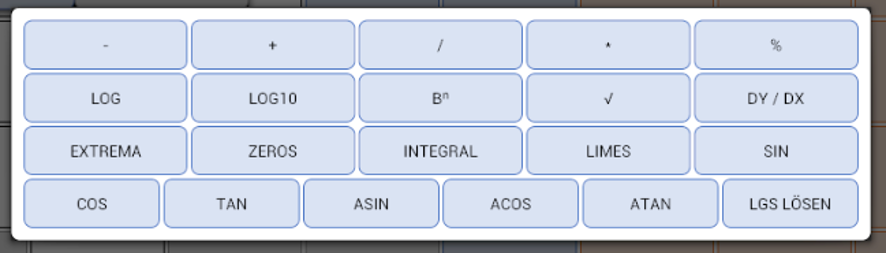
\includegraphics[width=\columnwidth]{img/inputtilemapping-for-operators}
	\caption[InputTileMapping for Operators]{InputTileMapping for Operators\footnotemark}
\end{figure}
\footnotetext{eigene Darstellung}

Im Kontrast zu den vielen Kacheldefinitionen, die es in \code{TileMapping} zu Einstellungen oder Operatoren gibt, findet man dort für den Stack und die Historie lediglich eine Definition wieder. (\code{S\_STACK}, \code{H\_HISTORY})

Was bei der Erstellung von sowohl Stack, als auch Historie von Relevanz ist, ist der Rang der Kachel. Dieser legt gemäß \code{TileScheme}-Definition fest, zu welchem Zeitpunkt Daten hineingeschoben oder gelöscht werden. Im \code{InputTileMapping} wird also für jeden möglichen Position in der Liste ein Eintrag angelegt. Gemäß der, vom \code{InputMenuFactory} erstellten Listener, wird dann das Historie- bzw. Stack-Tile an die ausgewählte Stelle gesetzt.

\begin{figure}[h]
	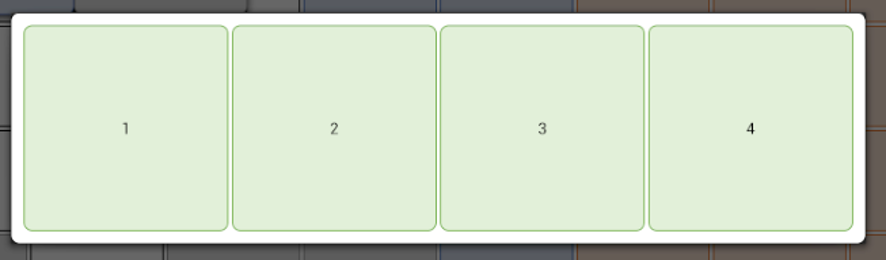
\includegraphics[width=0.7\columnwidth]{img/inputtilemapping-for-stack-with-3-tiles}
	\caption[InputTileMapping for Stack with 3 tiles]{InputTileMapping for Stack with 3 tiles\footnotemark}
\end{figure}
\footnotetext{eigene Darstellung}
\FloatBarrier

\paragraph{Klasse: InputDouble [Gentges]}

Für die Applikationen werden folgende Operanden (\code{ODouble}, \code{OFraction} und \code{OPolynom}) für die Eingabe vom User möglich sein. Die XML-Ansicht ist simpel gehalten und verwendet ein \code{RelativeLayout}, welches die relative Position zu den einzelnen Objekte verwendet. Dadurch wird die Layout-Hierarchie reduziert und die Performance der Applikation verbessert. Für das Eingabefeld wird ein \code{EditText} verwendet, das als Eingabetyp Dezimalzahlen unterstützt wird. In Android muss hier noch explizit erwähnt werden, dass erst über den Keyword \code{numberSigned} auch die Eingabe von negative Zahlen möglich ist.

\begin{figure}[h]
	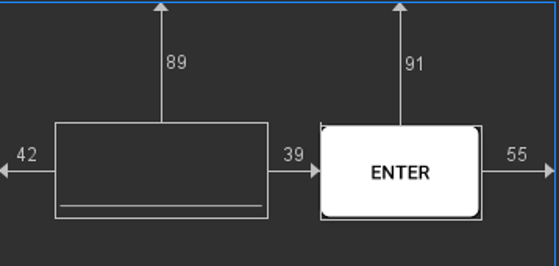
\includegraphics[width=0.6\columnwidth]{img/xml_InputDouble}
	\caption[XML-Designer für die Klassen InputDouble]{XML-Designer für die Klasse InputDouble\footnotemark}
\end{figure}
\footnotetext{eigene Darstellung in Android Studio}
\FloatBarrier

Die korrespondierende Java-Datei liest nach dem Bestätigen des Buttons den Wert aus dem \code{EditText} und kreiert ein \code{ODouble}-Objekt. Dieses Objekt wird mit seinem zugehörigen \code{TileMapping} einem \code{TileScheme} zugewiesen. Das vorher ausgewählte \code{Tile} aktualisiert seinen \code{TileScheme}. Abschließend schließt der Konstruktor die Dialoge über die Methode \code{dismissAll()}, die vorher erklärt wurde.

\paragraph{Klasse: InputFraction [Gentges]}

Diese Klasse deckt die Funktionalität der Benutzereingabe von Brüchen. Dabei ähnelt sie der Klasse \code{InputDouble}. Die Unterschiede beruhen dahingehend, dass ein zweites \code{EditText} integriert wurde, um sowohl als Zähler als auch Nenner abzufragen. Der ausgewählten \code{Tile} wird respektiv ein \code{TileScheme} mit \code{OFraction} übergeben. 

\begin{figure}[h]
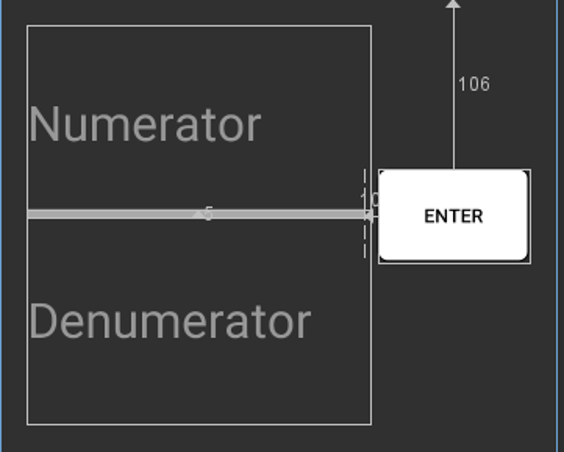
\includegraphics[width=0.5\columnwidth]{img/xml_InputFraction}
\caption[XML-Designer für die Klasse InputFraction]{XML-Designer für die Klasse InputFraction\footnotemark}
\end{figure}
\footnotetext{eigene Darstellung in AndroidStudio}
\FloatBarrier

\paragraph{Klasse: InputPolynomial [Gentges]}

Die Klasse ist grundsätzlich gleich aufgebaut, wie die vorherigen Eingabeklassen der Operanden. In der Abbildung lässt sich erkennen, dass die einzelne Polynome vom Nutzer eingegeben werden können.

\begin{figure}[h]
	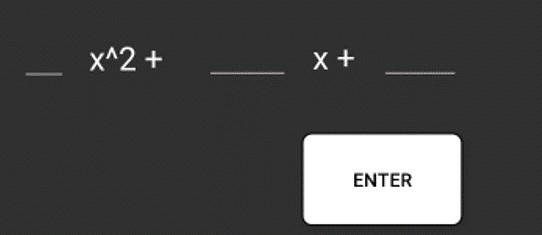
\includegraphics[width=0.6\columnwidth]{img/xml_InputPolynomial}
	\caption[XML-Designer für die Klasse InputPolynomial]{XML-Designer für die Klasse InputPolynomial\footnotemark}
\end{figure}
\footnotetext{eigene Darstellung in AndroidStudio}
\FloatBarrier
\clearpage

\paragraph{Die Beziehungen von den Menüsteuerungsklassen [Istogu]}

\begin{figure}[h]
	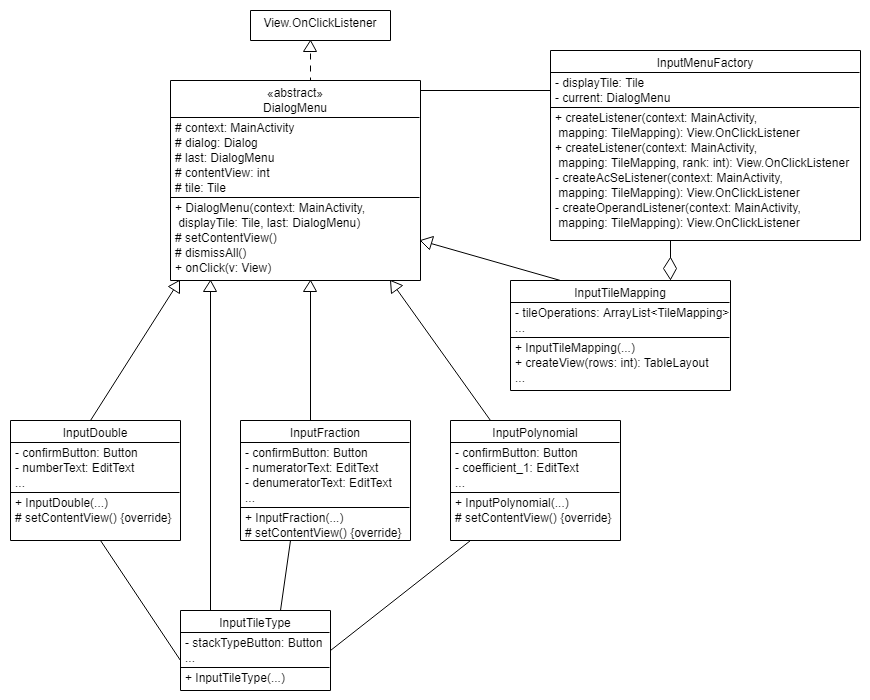
\includegraphics[width=\columnwidth]{img/klassendiagramm_Menusteuerung}
	\caption[Klassendiagramm: Menüsteuerung]{Klassendiagramm: Menüsteuerung\footnotemark}
\end{figure}
\footnotetext{eigene Darstellung}
\FloatBarrier

Wie aus dem Klassendiagramm entnommen werden kann, wurde die Menüsteuerung soweit wie möglich dynamisch gestaltet. Somit können dadurch weitere Funktionalitäten bzgl. Operanden bzw. Operationen hinzugefügt werden.  Zusätzlich sind die einzelne Menüs wie folgt gestaltet. Die einzelne Menüs bauen aufeinander und somit ist der Ablauf der einzelnen Menüs definiert. Abhängig von der ausgewählte Kachel werden \code{OnClickListener} gesetzt. Dies ist unter anderem aus dem Klassendiagramm bei der Implementierung von \code{View.OnClickListener} in der Klasse \code{DialogMenu} zu sehen. 
\clearpage

\subsection{Dokumentation der Models}

\subsubsection{Operanden [Schwenke]}

Für ein gut funktionierendes Backend ist ein einheitliches Datenmodel essenziell. So gibt es in der Kernbibliothek von Java einige Klassen für die Repräsentation von mathematischen Bausteinen, wie z.B. dem Bruch. Das gleiche gilt für \textit{Apache Commons Math}. 

Jedoch sind die meisten dieser Klassen sehr spezialisiert und miteinander nicht kompatibel. Deswegen wurde innerhalb des Projektteams entschieden für jeden unterstützten Operanden eine eigene Klasse zu erstellen, die jedoch alle von der gleichen abstrakten Klasse \code{Operand} erben sollen. 

Dadurch wird sichergestellt, dass es eine einheitliche Schnittstelle gibt, über die alle Operanden angesprochen werden können. Beschreiben kann man diese neuen Klassen auch als \textit{Wrapper}, da der Großteil der eigentlichen Funktionalitäten Teil der darunterliegenden Klassen ist. 

So soll z.B. \code{OMatrix} ein Wrapper um die Klasse \code{Array2DRowRealMatrix} sein. Damit kann man einerseits das einfache und einheitliche Interface nutzen und falls notwendig direkt auf das darunterliegende Objekt zugreifen, um spezielle Operationen durchführen zu können. 

Ein wichtiger Bestandteil dieser Wrapper sind auch die unterschiedlichen Konstruktoren. So kann jeder Operand aus einem einzelnen String konstruiert werden. 

Im Folgenden wird die gemeinsame Schnittstelle dargestellt. Gemeinsam haben alle diese Methoden, dass sie ohne Seiteneffekte auskommen. Statt das vorliegende Objekt zu verändern wird ein neues Objekt erstellt und zurückgegeben. Dies macht das Umkehren von Methodenaufrufen einfach. Man muss lediglich das zurückgegebene Objekt entfernen und das alte weiternutzen.

\paragraph{Klasse: Operand [Schwenke]}

\code{Operand turnAroundSign()}: Dreht alle Vorzeichen im Operand um. Erreicht wird das grundsätzlich durch Multiplikation mit \code{-1}. Konkreter muss dafür z.B. bei einer Matrix eine Multiplikation mit einem Skalar durchgeführt werden.

\code{Operand negateValue()}: Negiert den Operanden unabhängig von den Vorzeichen. Bei einer Matrix werden also alle Elemente negativ.

\code{Operand inverseValue()}: Die Inverse (wenn vorhanden) des jeweiligen Operanden wird berechnet.

\code{Boolean equalsValue(Operand o)}: Vergleicht den aktuellen Operanden mit einem übergebenen Operanden.

\code{String toString()}: Wandelt das Objekt in eine String-Repräsentation um.

\code{<T extends Object> get()}: Gibt das darunterliegende Objekt zurück. Im Falle von \code{OMatrix} ist dies eine \code{Array2DRowRealMatrix}. Bei einem Tupel ein \code{Array} von \code{Doubles}.

Auffallend ist hier der geringe Umfang der Schnittstelle der Operanden, da diese doch eigentlich die Grundlage für einen Taschenrechner bilden sollten. So kann man eine Matrix multiplizieren, addieren, dividieren und das alles in unterschiedlichsten Kombinationen mit anderen Arten von Operanden. Tatsächlich sind die meisten Kalkulationen – wie in der Projektplanung entworfen – in eigenen Klassen angelegt. Somit besteht eine Trennung zwischen Datenhaltung (den Operanden) und den Operationen, die auf den Daten ausgeführt werden können (Actions).

\paragraph{Klasse: ODouble [Meinerzhagen]}

\textit{Wrapper für ein} \code{Double}

Eine Dezimalzahl, welche intern einen \code{double} zur Datenspeicherung verwendet.


\paragraph{Klasse: OFraction [Meinerzhagen]}

\textit{Wrapper für Common Math Fraction}

Implementierung eines Bruchs. Die Zähler und Nenner sind durch \code{Doubles} umgesetzt. Im Gegensatz zu den meisten anderen Operanden gibt es hier mehr als zwei Konstruktoren. So kann man einmal Zähler und Nenner als zwei ganze Zahlen übergeben. Wird ein einzelnes \code{Double} übergeben, wird daraus automatisch ein Bruch erstellt. Alternativ kann direkt eine \code{Fraction} übergeben werden.

\paragraph{Klasse: OSet [Meinerzhagen]}

\textit{Wrapper für ein} \code{Double}-\code{Set}

Implementierung einer Menge. Das gleiche Element kann nicht mehrmals enthalten sein. Die Reihenfolge spielt keine Rolle. Umgesetzt ist die Klasse mit einem angepassten \code{Set}. Erstellen kann man ein \code{OSet} aus einem \code{Array} von \code{Doubles} oder einem String.

\paragraph{Klasse: OTuple [Meinerzhagen]}

\textit{Wrapper für ein} \code{Double}-\code{Array}

Implementierung eines Tupels. Das gleiche Element kann mehrmals enthalten sein. Die Reihenfolge spielt eine Rolle. Erstellen kann man ein \code{OTuple} aus einer übergebenen Liste oder einem String.

\paragraph{Klasse: OMatrix [Meinerzhagen]}

\textit{Wrapper für eine Apache Commons} \code{Array2DRowRealMatrix}

Implementierung einer Matrix. Das darunterliegende Objekt ist eine \code{RealMatrix}, die wiederrum eine \code{Array2DRowRealMatrix} enthält. Die Matrix an sich ist in einem zweidimensionalen Array von \code{Doubles} umgesetzt. Erstellen kann man eine \code{OMatrix} aus einem String oder einem zweidimensionalen \code{Array} von \code{Doubles}.


\paragraph{Klasse: OPolynom [Meinerzhagen]}

\textit{Wrapper für eine Apache Commons} \code{PolynomialFunction}

Implementierung eines Polynoms. Grundsätzlich entspricht das Polynom einer Sequenz von Dezimalzahlen. Abhängig von der Position in der Sequenz entscheidet sich, was der Exponent der jeweiligen Dezimalzahl ist. Somit müssen Funktionen immer in dieser Normalform vorliegen. Erstellen kann man ein \code{OPolynom} aus einem String oder einem \code{Array} von \code{Doubles}.

\paragraph{Klasse: OEmpty [Meinerzhagen]}

\textit{Leerer Wrapper}

Ein leerer Operand. Da alle \code{Operand}-Klassen Wrapper sind, ist technisch auch ein leerer Wrapper notwendig. Die hier implementierten Methoden aus der Schnittstelle stellen lediglich \textit{Stubs} dar und haben keine Funktion.

\paragraph{Klasse: DoubleFormatter [Meinerzhagen]}

Zentrale Anlaufstelle um \code{Doubles} in einen formattierten String umzuwandeln. Die einzige hier enthaltene Methode wird verwendet, um die Darstellung der Doubles zu vereinheitlichen. 

\code{String format(double d)}

\paragraph{Klasse: DoubleComparator [Meinerzhagen]}

Dezimalzahlen sind in den meisten Sprachen in dem IEE 754 Format implementiert. Das hat zur Folge, dass Konversionen und Änderungen einer konkreten Dezimalzahl zu Rundungsfehlern führen. Das ist auch in Java der Fall. Möchte man nun die beiden Dezimalzahlen \code{1.1} und \code{1.1} mit der Standardmethode in Java vergleichen, wird man in fast allen Fällen ein \code{false} zurückbekommen. Das liegt an den zuvor angesprochenen Rundungsfehlern. 

Da innerhalb dieses Projektes alles auf \code{Doubles} basiert ist es notwendig für dieses Problem eine Lösung zu finden. Dafür wurde diese Klasse entwickelt. Alle Vergleiche müssen über diese Klasse erfolgen.

\code{Boolean isEqual(double d1, double d2)} vergleicht zwei \code{Doubles} miteinander. Dies erfolgt über ein Delta. Zunächst wird die Differenz zwischen beiden Zahlen berechnet und anschließend überprüft, ob die Differenz unter einer definierten Grenze liegt. Alle weiteren Methoden in dieser Klasse benutzen diese Methode.

Weitere Methoden vergleichen \code{Arrays} und \code{Sets} miteinander.

\subsubsection{Operationen}

\paragraph{Klasse: Plus [Falk]}

\textbf{Eingabeparameter: }Zwei Werte, der erste Wert ist der erste Summand, der zweite der zweite Summand. Die erlaubten Kombinationen sind: 

\begin{itemize}
	\item \code{ODouble} und \code{ODouble}
	\item \code{ODouble} und \code{OFraction}
	\item \code{OFraction} und \code{ODouble}
	\item \code{ODouble} und \code{OSet}
	\item \code{OSet} und \code{ODouble}
	\item \code{ODouble} und \code{OMatrix}
	\item \code{OMatrix} und \code{ODouble}
	\item \code{ODouble} und \code{OPolynom}
	\item \code{OPolynom} und \code{ODouble}
	\item \code{ODouble} und \code{OTupel}
	\item \code{OTupel} und \code{ODouble}
	\item \code{OFraction} und \code{OFraction}
	\item \code{OFraction} und \code{OSet}
	\item \code{OSet} und \code{OFraction}
	\item \code{OFraction} und \code{OMatrix}
	\item \code{OMatrix} und \code{OFraction}
	\item \code{OFraction} und \code{OPolynom}
	\item \code{OPolynom} und \code{OFraction}
	\item \code{OFraction} und \code{OTuple}
	\item \code{OTupel} und \code{OFraction}
	\item \code{OMatrix} und \code{OMatrix}
	\item \code{OPolynom} und \code{OPoylnom}
	\item \code{OTuple} und \code{OTuple}
\end{itemize}

\textbf{Rückgabewerte: }Der berechnete Wert mit dem Datentyp des ersten Summanden. 

\textbf{Beschreibung: }Die Klasse verfügt über 23 öffentlich ansprechbare Methoden. Je nach übergebenen Parametern wird bestimmt, welche öffentliche Methode gemeint ist. Anschließend wird die Berechnung durchgeführt. 

\paragraph{Klasse: Minus [Falk]}

\textbf{Eingabeparameter: }Zwei Werte, der erste Wert ist der Minuend, der zweite der Subtrahend. Die erlaubten Kombinationen sind: 

\begin{itemize}
	\item \code{ODouble} und \code{ODouble} 
	\item \code{ODouble} und \code{OFraction}
	\item \code{OFraction} und \code{OFraction} 
	\item \code{OFraction} und \code{ODouble}
	\item \code{OSet} und \code{ODouble}
	\item \code{OSet} und \code{OFraction }
	\item \code{OMatrix} und \code{OMatrix}
	\item \code{OMatrix} und \code{ODouble}
	\item \code{OMatrix} und \code{OFraction}
	\item \code{OPolynom} und \code{OPolynom }
	\item \code{OPolynom} und \code{ODouble}
	\item \code{OPolynom} und \code{OFraction }
	\item \code{OTuple} und \code{OTuple}
	\item \code{OTuple} und \code{ODouble}
	\item \code{OTuple} und \code{OFraction}
\end{itemize} 

\textbf{Rückgabewerte: }Der berechnete Wert mit dem Datentyp des ersten, übergebenen Wertes. 

\textbf{Beschreibung: }Die Klasse verfügt über 15 öffentlich ansprechbare Methoden. Je nach übergebenen Parametern wird bestimmt, welche öffentliche Methode gemeint ist. Anschließend wird die Berechnung durchgeführt. 

\paragraph{Klasse: Minus [Falk]}

\textbf{Eingabeparameter: }Zwei Werte, der erste Wert ist der Dividend, der zweite der Divisor. Die erlaubten Kombinationen sind: 

\begin{itemize}
	\item \code{ODouble} und \code{ODouble}
	\item \code{ODouble} und \code{OFraction}
	\item \code{OFraction} und \code{OFraction} 
	\item \code{OFraction} und \code{ODouble} 
	\item \code{OSet} und \code{ODouble}
	\item \code{OSet} und \code{OFraction}
	\item \code{OMatrix} und \code{ODouble}
	\item \code{OMatrix} und \code{OFraction}
	\item \code{OPolynom} und \code{OPolynom}
	\item \code{OPolynom} und \code{ODouble}
	\item \code{OPolynom} und \code{OFraction}
	\item \code{OTuple} und \code{OTuple}
	\item \code{OTuple} und \code{ODouble}
	\item \code{OTuple} und \code{OFraction} 
\end{itemize}

\textbf{Rückgabewerte:} Der berechnete Wert mit dem Datentyp des ersten, übergebenen Wertes.
 
\textbf{Beschreibung: }Die Klasse verfügt über 14 öffentlich ansprechbare Methoden. Je nach übergebenen Parametern wird bestimmt, welche öffentliche Methode gemeint ist. Bevor die Berechnung durchgeführt wird, wird bestimmt ob der Divisor \code{0} ist. Wenn ja wird eine Fehlermeldung ausgegeben. Andernfalls wird die Berechnung durchgeführt. 

\paragraph{Klasse: Times [Falk]}

\textbf{Eingabeparameter:} Zwei Werte, der erste Wert ist der Multiplikator, der zweite Wert der Multiplikand. Die erlaubten Kombinationen sind: 

\begin{itemize}
\item \code{ODouble} und \code{ODouble}
\item \code{ODouble} und \code{OFraction}
\item \code{OFraction} und \code{ODouble}
\item \code{ODouble} und \code{OSet}
\item \code{OSet} und \code{ODouble}
\item \code{ODouble} und \code{OMatrix}
\item \code{OMatrix} und \code{ODouble}
\item \code{ODouble} und \code{OPolynom}
\item \code{OPolynom} und \code{ODouble}
\item \code{ODouble} und \code{OTupel}
\item \code{OTupel} und \code{ODouble}
\item \code{OFraction} und \code{OFraction}
\item \code{OFraction} und \code{OSet}
\item \code{OFraction} und \code{OMatrix}
\item \code{OMatrix} und \code{OFraction}
\item \code{OFraction} und \code{OPolynom}
\item \code{OFraction} und \code{OTupel}
\item \code{OMatrix} und \code{OMatrix}
\item \code{OPolynom} und \code{OPolynom} 
\item \code{OTupel} und \code{OTupel}
\end{itemize}

\textbf{Rückgabewerte: }Der berechnete Wert. 

\textbf{Beschreibung: }Die Klasse verfügt über 20 öffentlich ansprechbare Methoden. Je nach übergebenen Parametern wird bestimmt, welche öffentliche Methode gemeint ist. Anschließend wird die Berechnung durchgeführt. 

\paragraph{Klasse: Root [Falk]}

\textbf{Eingabeparameter: }Zwei Werte, der erste Wert ist der Radikand, der zweite Wert der Wurzelexponent. Die erlaubten Kombinationen sind: 

\begin{itemize}
\item \code{ODouble} und \code{ODouble}
\item \code{ODouble} und \code{OFraction}
\item \code{OFraction} und \code{ODouble} 
\item \code{OFraction} und \code{OFraction}
\item \code{OMatrix} und \code{ODouble}
\item \code{OMatrix} und \code{OFraction}
\end{itemize}

\textbf{Rückgabewerte:} Der berechnete Wert, Datentyp ist der des Radikanden. 

\textbf{Beschreibung: }Die Klasse verfügt über 6 öffentliche Methoden. Anhand der übergebenen Parameter wird bestimmt, welche öffentliche Methode aufgerufen wird. In der Methode wird die Wurzel berechnet und zurückgegeben. 

\paragraph{Klasse: Modulo [Falk]}

\textbf{Eingabeparameter:} Zwei Werte des Typs \code{ODouble}, der erste Wert ist der Dividend, der zweite der Divisor. 

\textbf{Rückgabewerte:} Der berechnete Wert als \code{ODouble}. 

\textbf{Beschreibung:} Die Klasse verfügt über eine öffentliche Methode. In der Methode wird der Modulo-Wert der beiden übergebenen Parameter berechnet. 

\paragraph{Klasse: Zeros [Keienburg]}

\textbf{Eingabeparameter: }Eine Funktion des Typs \code{OPolynom}

\textbf{Rückgabewerte:} Ein Set des Typs \code{OSet} mit den berechneten Nullstellen. Die Nullstellen werden als \code{Set} zurückgegeben, da so verhindert wird das für Funktionen wie \code{x\^{}2+0*x+0} zweimal die gleiche Nullstelle zurückgegeben wird. 

\textbf{Einstieg in die Klasse:} Öffentliche Methode, die die übergebenen Parameter entgegennimmt. Die weiteren Methoden für die Berechnung werden anschließend von der öffentlichen Methode aus aufgerufen. 
Methoden der Klasse \code{Zeros}:

\code{calculateZeros}: Die Methode erhält eine Funktion vom Typ \code{OPolynom}. Anschließend wird bestimmt, von welchem Grad die übergebene Funktion ist. Wenn die Funktion ersten Grades ist, wird die Methode \code{zerosTypeOne} aufgerufen, ansonsten die Methode \code{zerosTypeTwo}. Die beiden Methoden geben die gefundenen Nullstellen als 
Array zurück, das Array wird anschließend von \code{calculateZeros} zurückgegeben.
 
\code{normalOrQuadraticFunction}: Bestimmt, ob eine, als \code{Double} Array übergebene Funktion, ersten oder zweiten Grades ist. Dabei wird die Länge des Arrays getestet. Ist die Länge des Arrays 3, so wird die Funktion als Quadratische Funktion bestimmt. Wenn die Länge 2 ist, als einfache Funktion. 

\code{zerosTypeOne}: Die Methode berechnet die Nullstellen für Funktionen ersten Grades. Die Funktion wird als Double Array übergeben. Die berechnete Nullstelle wird als Double Array zurückgegeben. 

\code{zerosTypeTwo}: Die Methode berechnet die Nullstellen für Funktionen zweiten Grades. Die Funktion wird als Double Array übergeben. Mithilfe der Mitternachtsformel wird die erste und die zweite Nullstelle bestimmt. Die gefundenen Nullstellen werden als Double Array zurückgegeben. 

\textbf{Anmerkung:} Wenn eine übergebene Funktion keine Nullstellen besitzt, der Rückgabewert in Java also \code{NaN} ist, wird eine Fehlermeldung ausgegeben, dass eine Nullstellenberechnung nicht möglich ist. 

\textbf{Einschränkungen:} Die Nullstellenberechnung ist nur für Funktionen ersten und zweiten Grades möglich. 

Unit-Tests für die Klasse: 

\begin{enumerate}
	\item Eingabe Funktion: \code{2x + 4}. Erwartetes Ergebnis: \code{(-2)}
	\item Eingabe Funktion: \code{2x\^{}2+4x+0}. Erwartetes Ergebnis: \code{(-2, 0)}
	\item Eingabe Funktion: \code{x\^{}2+4x-4}. Erwartetes Ergebnis: \code{(-4,828, 0,828)}
\end{enumerate}

Die Tests waren erfolgreich.

\paragraph{Klasse: HighAndLowPoints [Keienburg]}

\textbf{Eingabeparameter:} Eine Funktion des Typs \code{OPolynom}

\textbf{Rückgabewerte: }Ein Tupel des Typs \code{OTupel} mit den berechneten Extremwerten. Die Werte an den geraden Positionen innerhalb des Tupels sind die X-Werte, der jeweils folgende Wert ist der zugehörige Y-Wert. Bsp.: Tupel [0] = X-Wert des ersten Extremwertes, Tupel [1] = Y-Wert des ersten Extremwertes, Tupel [2] = X-Wert des zweiten Extremwertes, Tupel [3] = Y-Wert des zweiten Extremwertes. 

Beschreibung: Die Klasse erhält eine Funktion vom Typ \code{ODouble}. Zuerst wird die Ableitung der Funktion bestimmt, anschließend die Nullstellen der Abteilung. Für die erhaltenen Nullstellen wird der zugehörige Y-Wert berechnet. Die berechneten Werte werden als \code{OTupel} zurückgegeben. 

Einstieg in die Klasse: Öffentliche Methode, die die übergebenen Parameter entgegennimmt. Die weiteren Methoden für die Berechnung werden anschließend von der Öffentlichen Methode aus aufgerufen. 

\textbf{Methoden der Klasse \code{HighAndLowPoints}:}

\code{getHighAndLowPoints}: Einstiegspunkt der Klasse, ruft die Methode \code{calculate}\linebreak\code{HighAndLowPoints} für die weitere Berechnung der Extremwerte auf. Gibt sie als \code{Double}-\code{Array} zurück. 

\code{getFunctionAsDouble}: Wandelt eine übergebene Funktion vom Typ \code{OPolynom} in ein Double Array um.

\code{calculateHighAndLowPoints}: Berechnet die Nullstellen einer übergebenen Funktion vom Typ \code{OPolynom}. Berechnet zuerst die Ableitung der Funktion, anschließend die Nullstellen der Ableitung. Die Werte der Nullstellen werden anschließend in die ursprüngliche Funktion eingesetzt und so die Y-Werte berechnet. Die berechneten Nullstellen werden als Double Array zurückgegeben. 

\code{Einschränkungen}: Die Nullstellenberechnung ist nur für Funktionen zweiten Grades möglich. Demnach ist eine Berechnung der Hoch- und Tiefpunkte nur für Funktionen dritten oder zweiten Grades möglich.

Unit-Tests für die Klasse:

\begin{enumerate}
\item Eingabe Funktion: 2x\^{}2+4x+6. Erwartetes Ergebnis: (-1|4)
\item Eingabe Funktion: 3x\^{}2+6x-4. Erwartetes Ergebnis: (-1|-7)
\item Eingabe Funktion: -2*x\^{}2+4x+12. Erwartetes Ergebnis: (1|14)
\end{enumerate}

Die Tests waren erfolgreich.

\paragraph{Logarithm [Keienburg]}

\textbf{Eingabeparameter:} Ein Wert des Typs \code{ODouble} oder zwei Werte vom Typ \code{ODouble} (erster ist die Basis) 

\textbf{Rückgabewerte:} Ein Wert des Typs \code{ODouble}

\textbf{Beschreibung:} Die Klasse berechnet den Logarithmus. Die Art des Logarithmus ist abhängig von den übergebenen Parametern. Wird nur ein Wert übergeben, wird der natürliche Logarithmus der Zahl berechnet. Wenn zwei Parameter übergeben werden, ist der erste Parameter die Basis des Logarithmus, der zweite der Wert, für den der Logarithmus berechnet werden soll. 

Der Einstieg in die Klasse erfolgt über zwei öffentliche Methoden. Die Methode wird anhand der übergebenen Parameter (ein oder zwei Werte vom Typ \code{ODouble}) ausgewählt. In der Öffentlichen Methode findet die Berechnung des Logarithmus (Natürlicher oder Logarithmus zu einer bestimmten Basis) statt. Wenn ein Wert kleiner gleich null eingegeben wird, wird eine Fehlermeldung ausgegeben.

Unit-Tests für die Klasse: 4 Unit-Test für die Berechnung der des natürlichen Logarithmus (ersten 4), 3 Unit-Tests für die Berechnung des Logarithmus für eine beliebige Basis. 

\begin{enumerate}
\item Eingabe 10. Erwartetes Ergebnis: 2.302585092994046
\item Eingabe: 5. Erwartetes Ergebnis: 1.6094379124341003
\item Eingabe: 97. Erwartetes Ergebnis: 4.574710978503383
\item Eingabe: e. Erwartetes Ergebnis: 1
\item Eingabe: Basis 5, Wert 10. Erwartetes Ergebnis: 1.4306765580733933
\item Eingabe: Basis 10, Wert 10. Erwartetes Ergebnis: 1
\item Eingabe: Basis e, Wert 10. Erwartetes Ergebnis: 2.302585092994046
\end{enumerate}

Die Tests waren erfolgreich.

\paragraph{Logarithm10 [Keienburg]}

\textbf{Eingabeparameter:} Ein Wert des Typs \code{ODouble}

\textbf{Ausgabeparameter:} Ein Wert des Typs \code{ODouble}

\textbf{Beschreibung:} Die Klasse berechnet den Logarithmus zur Basis 10. Wenn ein Wert kleiner gleich 0 eingegeben wird, wird eine Fehlermeldung ausgegeben. 

Unit-Tests für die Klasse: 

\begin{enumerate}
\item Eingabe 10. Erwartetes Ergebnis: 1
\item Eingabe: 5. Erwartetes Ergebnis: 0.6989700043360189
\item Eingabe: 97. Erwartetes Ergebnis: 1.9867717342662448
\end{enumerate}

Die Tests waren erfolgreich.

\paragraph{Derivation [Keienburg]}

\textbf{Eingabeparameter: }Eine Funktion des Typs \code{OPolynom}

\textbf{Rückgabewert:} Eine Funktion des Typs \code{OPolynom}

\textbf{Beschreibung:} Die Klasse berechnet die Ableitung zu einer übergebenen Funktion des Typs \code{OPolynom} und gibt sie als Funktion vom Typ \code{OPolynom} zurück. 

\textbf{Einstieg in die Klasse: }Öffentliche Methode, die die übergebenen Parameter entgegennimmt. Die weiteren Methoden für die Berechnung werden anschließend von der Öffentlichen Methode aus aufgerufen. 

\textbf{Methoden der Klasse Derivation: }

\code{getFunctionAsDouble:} Wandelt eine gegebene Funktion vom Typ \code{OPolynom} in ein \code{Double}-\code{Array} um. 

\code{derivate: }Berechnet die Ableitung einer gegebenen Funktion. Die Funktion wird zuerst in ein \code{Double}-\code{Array} umgewandelt, anschließend abgeleitet und als Funktion vom Typ \code{OPolynom} zurückgegeben. 

Unit-Tests für die Klasse: 

\begin{enumerate}
\item Eingabe 2x\^{}2+4x+6. Erwartetes Ergebnis: 4x+4
\item Eingabe: 7x+9. Erwartetes Ergebnis: 7
\item Eingabe: 12x\^{}2-3+12. Erwartetes Ergebnis: 24x-1
\item Eingabe: 1.5x\^{}2+2x+7. Erwartetes Ergebnis: 2.25x+2
\end{enumerate}  

Die Tests waren erfolgreich.

\paragraph{Integral [Istogu]}

Diese Klasse erbt von der Klasse \code{Action}. Daher sind die Methoden \code{with() }bereits implementiert. Diese Klasse berechnet entweder die Stammfunktion von dem übergebene Polynomialfunktion oder das Integral der Funktion. 

Für die Bildung der Stammfunktion benötigt die Methode \code{getAntiderivative()} eine \code{OPolynom} und gibt die Stammfunktion als Typ \code{OPolynom} zurück. Beim Aufleiten entsteht eine Konstante, die jede Wert annehmen kann. In der App wird festgelegt, dass diese Konstante immer 0 ist. Zweck hinter der Definition ist, dass mit dem \code{OPolynom} weitergerechnet werden kann, da diese nicht mit weiteren Variablen arbeiten kann.

Für das Berechnen des Integrals \code{getSimpsonIntegrator()} werden folgende Parametertypen erwartet: 

\begin{itemize}
	\item \code{OPolynom oPolynom}
	\item \code{double lowerBound}
	\item \code{double upperBound}
\end{itemize}

Das Integral für den vorgegebenen Bereich wird als \code{ODouble} zurückgegeben. Diese Methode realisiert die Simpsonregel für die Integration von reellen Funktionen, die in dem genutzten Mathebibliothek als Klasse \code{SimpsonIntegrator} implementiert wurde. 

Nach der Implementierung der Klasse erstellte ich dazu gehörig eine Unit-Test-Klasse. Im Nachfolgenden werden die Ergebnisse dargestellt, die alle erfolgreich waren. 

\code{getSimpsonsIntegrator()}

\quad \quad \textbf{ Eingabe:} \code{OPolynom}: \code{x\^{}2 – 8x + 17}, untere Grenze: 2, obere Grenze 5

\quad \quad \textbf{Erwartetes Ergebnis:} 6

\code{getAntiderivative()}

\quad \quad \textbf{Eingabe:} \code{OPolynom}: \code{-3,21x\^{}3 + 3x + 7}

\quad \quad \textbf{Erwartetes Ergebnis}: \code{OPolynom}: \code{-0,8025x\^{}4 + 1,5x\^{}2 + 7x + c}

\vspace{1em}

\paragraph{Bestimmung des Grenzwertes einer Funktion [Istogu]}

Für die Umsetzung wurde die Funktion \code{value(double x)} der Klasse \code{PolynomialFunction} verwendet, die aus der Mathebibliothek \textit{Apache Commons Math} hervorgeht. Zudem bietet die \code{Double}-Klasse die Repräsentierung von positiv und negativ Unendlich an, die auch für die Methoden verwendet wurde.

Für die Bestimmung des Grenzwertes wurde sich an der Methode der numerischen Annäherung orientiert. Hierbei wird der Grenzwert durch die Annäherung von links und rechts des untersuchten Punktes bestimmt. Daher wurde die Anforderung in drei Methoden untergliedert, einmal die Methode \code{limitFromBelow(…)} und \code{limitFromAbove(…)}, die jeweils die Annäherung von verschiedenen Richtungen bestimmt. Die Rückgabewerte der beiden Methoden werden in der Methode \code{limit(…)} miteinander verglichen. Zweck der Vergleichsabfrage ist es Definitionslücken abzufangen. Als Beispiel wird folgende Funktion angenommen:

\[f(x) = \frac{1}{x}\]

\begin{figure}[!h]
	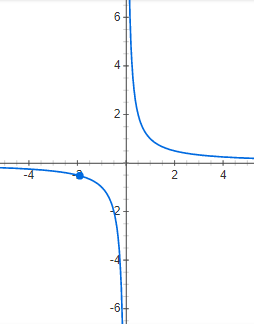
\includegraphics[scale=1]{img/funktion-grafik}
	\caption[Grafische Darstellung der Funktion]{Grafische Darstellung der Funktion\footnotemark}
\end{figure}
\footnotetext{Darstellung von der Googlesuche}

Wenn für die Funktion sowohl der linksseitige als auch der rechtsseitige Grenzwert bestimmt wird, folgt folgendes:  

%$\lim_{x\to\0+} \frac{1}{x}\ = infty$

%$\lim_{x\to\0-} \frac{1}{x}\ = - infty$


Wenn der linksseitige und rechtsseitige Grenzwert nicht übereinstimmen, ist der Grenzwert an dieser Stelle nicht existent. In dem Fall beruht es darauf, dass das Ergebnis einer Division mit dem Divisor null nicht definiert ist. Solche Unstimmigkeiten können unter anderem auch in abschnittsweise definierten Funktionen vorkommen, die im Funktionsumfang der App nicht integriert sind. Trotz dessen werden solche Fälle mit dem Vergleich zwischen dem linksseitigen und rechtsseitigen Grenzwert in der Methode \code{limit(…)} berücksichtigt.

Für die jeweilige Annäherung wurde die Überlegung getätigt, welche Fälle in der Grenzwertbestimmung von Funktionen vorkommen können. Dabei wurden folgende Lösungsmöglichkeiten festgestellt:
\begin{itemize}
	\item Positiv unendlich
	\item Negativ unendlich
	\item Nicht definiert
	\item \code{xxx} war Zeichen (Ubiquator Teilmenge von Realer Zahlenraum)
\end{itemize}

Darauf aufbauend wurde ein Struktogramm angefertigt, auch als Nassi-Shneiderman-Diagramm bekannt. Dabei wird die Annäherung von unten veranschaulicht, weil die Annäherung von oben nach dem gleichen Grundprinzip erfolgt. 

\begin{figure}[!h]
	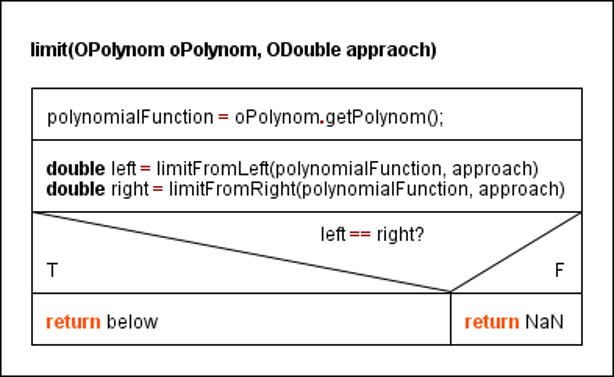
\includegraphics[scale=1]{img/struktogramm-limit}
	\caption[Struktogramm für die Methode limit]{Struktogramm für die Methode limit\footnotemark}
\end{figure}
\footnotetext{eigene Darstellung}
\FloatBarrier


\begin{figure}[!h]
	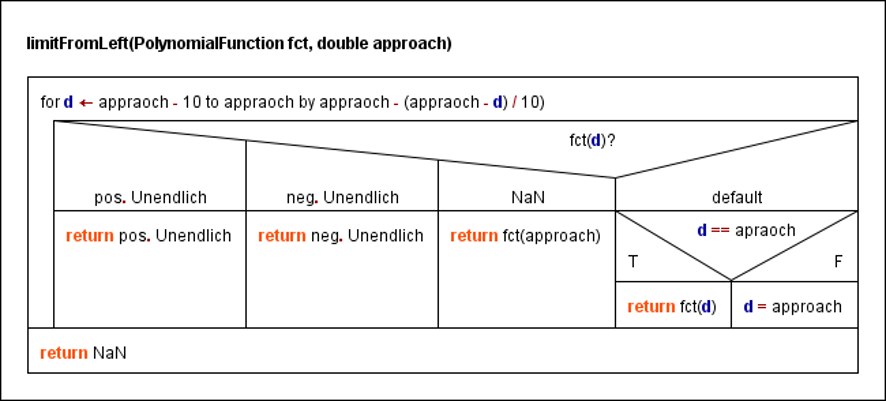
\includegraphics[scale=1]{img/struktogramm-limitFromLeft}
	\caption[Struktogramm für die Methode limitFromLeft]{Struktogramm für die Methode limitFromLeft\footnotemark}
\end{figure}
\footnotetext{eigene Darstellung}
\FloatBarrier

Die Klasse \code{Limes} erbt von der Klasse \code{Action}. Dahin gehend besitzt die Klasse die Methode \code{with()}, welche die Methode \code{on()} aufruft. Da diese Klasse keine Methodenüberladung für \code{on()} hat, wird kein Nutzen durch diese Art der Implementierung gewonnen, jedoch bietet es die Möglichkeit der Erweiterung an. In der Methode \code{on()} wird die Methode \code{limit()} aufgerufen.

\textbf{Methode:} \code{on()}

\textbf{Eingabeparameter: }Objekt des Typs \code{OPolynom}, Wert (Stelle an der, der Grenzwert berechnet wird) des Typs \code{ODouble}

\textbf{Rückgabewerte: }Einzelner Wert des Typs \code{ODouble}

Nach der Implementierung der Klasse wurde die dazu gehörig eine Unit-Test-Klasse erstellt. Im Nachfolgenden werden die Ergebnisse dargestellt, die alle erfolgreich waren.

\begin{enumerate}
	\item Eingabe: \code{OPolynom}: x\^{}2 + 1, Stelle: 26 \\
	Erwartetes Ergebnis: 26 
	\item Eingabe: -0.3333x\^{}3 + 2x, Stelle: pos. Unendlich \\
	Erwartetes Ergebnis: neg. Unendlich
	\item Eingabe: 3x\^{}3, Stelle: pos. Unendlich \\
	Erwartetes Ergebnis: pos. Unendlich
\end{enumerate}

\paragraph{Klasse: Sinus [Keienburg]}
\textbf{Eingabeparameter: } Einzelner Wert des Typs \code{ODouble}

\textbf{Rückgabewerte: } Einzelner Wert des Typs \code{ODouble}

\textbf{Beschreibung: } Der Klasse wird ein Winkel vom Datentyp \code{ODouble} übergeben. Der Winkel wird in einen Wert des Typs \code{Double} konvertiert, anschließend mithilfe der Methode \code{Math.toRadians} in ein Winkelmaß. Von diesem Winkelmaß wird dann mit der Methode \code{Math.sin} der Sinus berechnet und als \code{ODouble} zurückgegeben.  

Die Klasse wird über eine Öffentliche Methode aufgerufen. In der Methode selbst wird der Sinus berechnet. 

Unit-Tests für die Klasse: 	
\begin{enumerate}
	\item Eingabe:  10 Erwartetes Ergebnis: 0.17364817766693033
	\item Eingabe:  45 Erwartetes Ergebnis: 0.7071067811865475
	\item Eingabe: -45 Erwartetes Ergebnis: -0.7071067811865475
\end{enumerate}
Die Tests waren erfolgreich.

\paragraph{Klasse: ArcSinus [Keienburg]}
\textbf{Eingabeparameter: } Einzelner Wert des Typs \code{ODouble}

\textbf{Rückgabewerte: } Einzelner Wert des Typs \code{ODouble}

\textbf{Beschreibung: } Der Klasse wird ein Winkel vom Datentyp \code{ODouble} übergeben. Der Winkel wird in einen Wert des Typs \code{Double} konvertiert, anschließend mithilfe der Methode \code{Math.toRadians} in ein Winkelmaß. Von diesem Winkelmaß wird dann mit der Methode \code{Math.asin} die Inverse des Sinus berechnet und als \code{ODouble} zurückgegeben.  

Die Klasse wird über eine Öffentliche Methode aufgerufen. In der Methode selbst wird der Arkussinus berechnet. 

Unit-Tests für die Klasse: 	
\begin{enumerate}
	\item Eingabe:  10 Erwartetes Ergebnis: 0.17543139267904395
	\item Eingabe:  45 Erwartetes Ergebnis: 0.9033391107665127
	\item Eingabe: -45 Erwartetes Ergebnis: -0.9033391107665127
\end{enumerate}
Die Tests waren erfolgreich.

\paragraph{Klasse: Cosinus [Keienburg]}
\textbf{Eingabeparameter: } Einzelner Wert des Typs \code{ODouble}
	
\textbf{Rückgabewerte: } Einzelner Wert des Typs \code{ODouble}
	
\textbf{Beschreibung: } Der Klasse wird ein Winkel vom Datentyp \code{ODouble} übergeben. Der Winkel wird in einen Wert des Typs \code{Double} konvertiert, anschließend mithilfe der Methode \code{Math.toRadians} in ein Winkelmaß. Von diesem Winkelmaß wird dann mit der Methode \code{Math.cos} der Cosinus berechnet und als \code{ODouble} zurückgegeben.  Die Klasse wird über eine Öffentliche Methode aufgerufen. In der Methode selbst wird der Cosinus berechnet. 
	
Unit-Tests für die Klasse: 	
\begin{enumerate}
	\item Eingabe:  10 Erwartetes Ergebnis: 0.984807753012208
	\item Eingabe:  45 Erwartetes Ergebnis: 0.7071067811865476
	\item Eingabe: -45 Erwartetes Ergebnis: -0.7071067811865476
\end{enumerate}
Die Tests waren erfolgreich.

\paragraph{Klasse: ArcCosinus [Keienburg]}
\textbf{Eingabeparameter: } Einzelner Wert des Typs \code{ODouble}

\textbf{Rückgabewerte: } Einzelner Wert des Typs \code{ODouble}

\textbf{Beschreibung: } Der Klasse wird ein Winkel vom Datentyp \code{ODouble} übergeben. Der Winkel wird in einen Wert des Typs \code{Double} konvertiert, anschließend mithilfe der Methode \code{Math.toRadians} in ein Winkelmaß. Von diesem Winkelmaß wird dann mit der Methode \code{Math.acos} die Inverse des Cosinus berechnet und als \code{ODouble} zurückgegeben.  

Die Klasse wird über eine Öffentliche Methode aufgerufen. In der Methode selbst wird der Arkuscosinus berechnet. 

Unit-Tests für die Klasse: 	
\begin{enumerate}
	\item Eingabe:  10 Erwartetes Ergebnis: 1.3953649341158527
	\item Eingabe:  45 Erwartetes Ergebnis: 0.6674572160283838
	\item Eingabe: -45 Erwartetes Ergebnis: 2.4741354375614093
\end{enumerate}
Die Tests waren erfolgreich.

\paragraph{Klasse: Tangens [Keienburg]}
\textbf{Eingabeparameter: } Einzelner Wert des Typs \code{ODouble}

\textbf{Rückgabewerte: } Einzelner Wert des Typs \code{ODouble}

\textbf{Beschreibung: } Der Klasse wird ein Winkel vom Datentyp \code{ODouble} übergeben. Der Winkel wird in einen Wert des Typs \code{Double} konvertiert, anschließend mithilfe der Methode \code{Math.toRadians} in ein Winkelmaß. Von diesem Winkelmaß wird dann mit der Methode \code{Math.tan} der Tangens berechnet und als \code{ODouble} zurückgegeben.  

Die Klasse wird über eine Öffentliche Methode aufgerufen. In der Methode selbst wird der Tangens berechnet. 

Unit-Tests für die Klasse: 	
\begin{enumerate}
	\item Eingabe:  10 Erwartetes Ergebnis: 0.17632698070846498
	\item Eingabe:  45 Erwartetes Ergebnis: 0.9999999999999999
	\item Eingabe: -45 Erwartetes Ergebnis -0.9999999999999999
\end{enumerate}
Die Tests waren erfolgreich.

\paragraph{Klasse: ArcTangens [Keienburg]}
\textbf{Eingabeparameter: } Einzelner Wert des Typs \code{ODouble}

\textbf{Rückgabewerte: } Einzelner Wert des Typs \code{ODouble}

\textbf{Beschreibung: }Der Klasse wird ein Winkel vom Datentyp \code{ODouble} übergeben. Der Winkel wird in einen Wert des Typs \code{Double} konvertiert, anschließend mithilfe der Methode \code{Math.toRadians} in ein Winkelmaß. Von diesem Winkelmaß wird dann mit der Methode \code{Math.atan} die Inverse des Tangens berechnet und als \code{ODouble} zurückgegeben. 
 
Die Klasse wird über eine Öffentliche Methode aufgerufen. In der Methode selbst wird der Arkustangens berechnet. 

Unit-Tests für die Klasse: 	
\begin{enumerate}
	\item Eingabe:  10 Erwartetes Ergebnis: 0.1727924348551592
	\item Eingabe:  45 Erwartetes Ergebnis: 0.6657737500283538
	\item Eingabe: -45 Erwartetes Ergebnis: -0.6657737500283538
\end{enumerate}
Die Tests waren erfolgreich.

\subsubsection{Lösen von Gleichungssystemen [Istogu]}

Da bereits die Grundrechenoperationen auch den Operand Matrix unterstützt, beschäftigt sich die Klasse \code{MatrixUtil} mit der Problemstellung ein lineares Gleichungssystem, die wie folgt aufgebaut ist.\footnote{\cite[vgl.][]{gordoncollegemathematicscomputersciencedepartment2019}}
\[A*x=b\]
zu lösen. Dabei ist A eine quadratische Matrix (n x n) und b ein Vektor (n).
Die Klasse besitzt eine ''on'' Methode, die dann solveLinearSystem() aufruft. Dabei erwartet die Methode ''on'' jeweils ein Objekt des Typs OMatrix und OTuple und gibt ein OTuple zurück. 

\begin{figure}[h]
	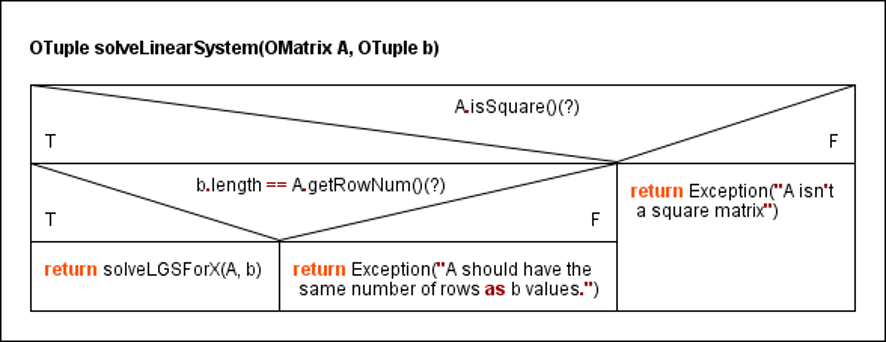
\includegraphics[width=\columnwidth]{img/solveLinearSystem}
	\caption[Struktogramm für die Methode solveLinearSystem]{Struktogramm für die Methode solveLinearSystem\footnotemark}
\end{figure}
\footnotetext{eigene Darstellung}

Aus der Abbildung geht die geplante bzw. realisierte Umsetzung für die Überprüfung der Parameter nach ihrer richtigen Form. 

Nach der Implementierung der Klasse erstellte ich dazu gehörig eine Unit-Test-Klasse. Im Nachfolgenden werden die Ergebnisse dargestellt, die alle erfolgreich waren. 
\begin{enumerate}
	\item Eingabe - Matrix: $$ A= \left(\begin{matrix}3&-7&0&-6\\2&-8&-1&4\\0&9&-7&9\\-4&5&-3&-8\end{matrix}\right) $$
  Eingabe - Vektor: $$ b= \left(\begin{matrix} 8\\1\\-7\\-1\end{matrix}\right) $$ Erwartetes Ergebnis: $$ x= \left(\begin{matrix} 1.197\\-0.1285\\0.0828\\-0.5849\end{matrix}\right) $$
	
\end{enumerate}


\subsubsection{Stackhandhabung [Keienburg]}

Ein integraler Bestandteil eines RPN-Taschenrechners stellt der Stack für die Haltung der Operanden dar. Im Rahmen der Projektplanung ist festgestellt worden, dass die in Java vorhandenen Implementationen eines Stacks die Anforderungen des Projekts nicht erfüllen. Gesondert genannt werden soll hier nochmals die Möglichkeit mit einer beliebigen Anzahl von Objekten auf dem Stack gleichzeitig zu arbeiten. Aufgrund dessen wurde entschieden eine eigene Umsetzung eines Stacks zu entwickeln. Der Entwurf des neuen Stacks erfolgte mithilfe der Java-Schnittstelle \code{StackInterface}, welche im Folgenden (leicht vereinfacht) dargestellt ist.

\begin{lstlisting}[caption=Stackinterface,label=list:stackinterface,language=Java]
void push(T value);
void push(T[] values);


T pop();\\
List<T> pop(int max);\\
<G extends T> G pop(Class<G> type);\\
<G extends T> List<G> pop(int max, Class<G> type);\\
T peek();\\
List<T> peek(int max); \\
<G extends T> G peek(Class<G> type); \\
<G extends T> List<G> peek(int max, Class<G> type); \\
boolean contains(T object); \\
void clear(); \\
T[] get(); \\
<G extends T> List<G> get(Class<G> type);\\
int size();
\end{lstlisting}

\code{T} und \code{G} werden in dem Interface als generische Typparameter genutzt. Das macht es möglich das Interface bzw. den Stack mit verschiedensten Implementationen zu nutzen. So kann man bei Bedarf nicht nur die einen Stack für Operanden, sondern auch für andere Klassen implementieren. Bei der Implementation wird der Typ-Paramter \code{T} durch eine konkrete Klasse (z.B. \code{Operand}, ersetzt. Ein Neuentwurf der Schnittstelle ist nicht notwendig. 

Der größte Unterschied zu anderen Stack-Interfaces ist, dass die drei bekannten Stack-Operationen \code{push}, \code{pop} und \code{peek} sowohl einzelne Parameter als auch Sammlungen von Parametern unterstützen. So kann man sich zum Beispiel die ersten 4 Objekte einer bestimmten Klasse mit einem einzigen Methodenaufruf von \code{pop} vom Stack entfernen. Bei einem normalen Stack sind eine ganze Reihe von Operationen dafür notwendig. Der Stack muss Element um Element auseinandergenommen, die ungewünschten Objekte entfernt, die anderen zwischengespeichert und anschließend wieder zusammengebaut werden.

Implementiert wird \code{StackInterface} von der Klasse \code{OperandStack}. Technisch ist der Stack als \code{LinkedList} umgesetzt. Um weitere Methoden außerhalb der \code{LinkedList}-Klasse auf dem Objekt nutzen zu können, wird das Objekt weiteren Klassenvariablen vom Typ \code{List} und \code{Deque} zugewiesen. Das ist möglich, weil all diese Klassen vom Typ \code{Collections} erben. Je nach Anforderung werden unterschiedliche Interfaces der \code{Collection} verwendet. So wird für ein klassisches \code{pop} das Interface einer \code{Deque} verwendet, während für ein \code{peek} bei dem die gewünschte Klasse und maximale Anzahl zurückgegebener Objekte angegeben werden kann, die Methoden einer \code{ArrayList} genutzt werden. So entsteht ein auf das Projekt optimal angepasstes Stack.

\subsubsection{Settings [Falk]}

Die meisten der Funktionen eines Taschenrechners wurden bereits beschrieben, doch nicht alle Funktionalitäten können mit der Kombination aus Operation und Operand beschrieben werden. So gibt es beispielsweise Sondertasten, die Eingaben manipulieren, besondere Operationen durchführen oder gänzlich von jeglicher Berechnung abweichen. Diese Sondertasten werden als Setting beschrieben und einem simplen, parameterfreiem Methodenaufruf angesprochen. Der Umgang mit dem erhaltenen Aufruf obliegt allein der implementierten Sondertaste.

\paragraph{Abstrakte Klasse: Setting}
\textit{Abstrakte Überklasse jeglicher Sondertasten und Settings}

Definiert die abstrakte Methode \code{call()}, die aufgerufen wird.
\paragraph{Klasse: \code{AllClear}}
\textit{AC}

Leert den gesamten aktuellen Input im Presenter
\paragraph{Klasse: DeleteEntry}
\textit{DELETE} 

Löscht den zuletzt eingegebenen Input
\paragraph{Klasse: ClearHistory}
\textit{CLEAR HISTORY}

Leert die gesamte Historie
\paragraph{Klasse: Enter}
\textit{ENTER}

Finalisiert eingegebene Operanden, sodass sie nicht mehr bearbeitet werden können und fügt sie zur Historie hinzu.
\paragraph{Klasse: Dot}
\textit{.}

Ermöglicht die Eingabe von Nachkommastellen am aktuellen Input.
\paragraph{Klasse: Inverse}
\textit{1/x}

Berechnet die Inverse des letzten Operanden im Stack.
\paragraph{Klasse: Split}
\textit{SPLIT}

Trennt Operanden vom Typ \code{OTuple}, \code{OSet} und \code{OMatrix} in einzelne Operanden vom Typ \code{ODouble}.
\paragraph{Klasse: Swap}
\textit{SWAP}

Tauscht die letzten beiden Operanden miteinander.
\paragraph{Klasse: ToTuple}
\textit{TO TUPLE}

Fügt so viele Operanden wie möglich zu einem \code{OTuple} Operand zusammen.
\paragraph{Klasse: TurnAroundSign}
\textit{+/-}

Vorzeichenwechselkriterium.
\paragraph{Klasse: LoadLayout}
\textit{LOAD LAYOUT}

Öffnet ein Menü zum Laden von Layouts.
\paragraph{Klasse: SaveLayout}
\textit{SAVE LAYOUT}

Öffnet ein Menü zum Speichern des aktuellen Layouts.


\subsubsection{Generische Kalkulationsorchestrierung [Schwenke]}

Wie schon im Kapitel zur Projektplanung erwähnt, stellt die Strukturierung und Architektur der Rechnungsumsetzung im Backend eine der vielen Anforderungen des Projektes dar. Identifiziert wurden zwei Hauptarten von Kalkulationen. 

Die erste Art ist generisch und wird in einer großen Anzahl benötigt. Ein Beispiel dafür ist die Addition. Da der Taschenrechner viele unterschiedliche Operanden-Typen unterstützt (Matrizen, Brüche, Mengen, usw.) sind enorm viele Methoden notwendig, um alle Möglichkeiten der Addition abdecken zu können. Auch muss irgendwo vom Programm entschieden werden, welche Methode genau aufgerufen werden soll. Statt dies mit komplexen If-Else-Bedingungen zu lösen, wurde in der Planungsphase entschieden Reflektion zu nutzen. Somit kann man in sich geschlossene kleine Methoden programmieren, die - sofern die Schnittstellenanforderungen erfüllt sind - automatisch erkannt und von der Reflektionsmethode aufgerufen werden können. Der Nutzer im Frontend muss lediglich entscheiden, was für eine Art von generischer Kalkulation er ausführen möchte. Zum Beispiel Addition oder Multiplikation. 

Die zweite Art von Kalkulationen sind sehr spezifisch, z.B. ein bestimmter Algorithmus zum Lösen von kubischen Gleichungen. Hier sind keine/kaum Kombinationen möglich und können somit direkt aufgerufen werden, ohne Reflektion zu verwenden.

Implementiert ist die Reflektion in der abstrakten Klasse \code{Action}. Die Klassenvariable \code{scopedAction} zeigt zur Laufzeit auf eine konkrete Implementierung einer \code{Action}, also z.B. \code{Plus}. Auf \code{scopedAction} wird die Reflektion ausgeführt. Letztere ist in der Methode \code{with()} umgesetzt. Diese stellt die Schnittstelle zu den generischen Kalkulationen erster Art dar. Hier ist der Methodenkopf zu sehen:

\begin{figure}[bht]
	\begin{lstlisting}[
	caption=Methodenkopf der generischen Schnittstelle,
	label=list:methodenkopf-der-generischen-schnittstelle,
	language=Java]
	@Contract(pure = true) public @NotNull 
	Operand with(@NotNull Operand... operands) 
	throws CalculationException
	\end{lstlisting}    
\end{figure}

Die erste Zeile definiert einige Eigenschaften der Methode. \code{@Contract} sagt aus, dass die Funktion \textit{pure} ist. Sie gibt für Tupel von Operanden immer das gleiche Ergebnis zurück und ist grundsätzlich ohne Nebeneffekte. Das ist hilfreich für das automatische Testen. Als Parameter wird ein beliebig gro"ses Array von Operanden übergeben. Das Ergebnis ist immer eine valide Instanz von \code{Operand}. Wird versucht eine nicht unterstützte Kalkulation auszuführen, wird \code{CalculationException} geworfen. Diese Ausnahme ist keine \code{RunTimeException} und muss deswegen explizit behandelt werden. Alternativ hätte man hier auch Optionals nutzen. Jedoch unterstützt die genutzte Version der Android API dieses Java-Feature nicht.

\begin{figure}[bht]
	\begin{lstlisting}[
	caption=Implementierung der generischen Schnittstelle,
	label=list:implementierung-der-generischen-schnittstelle,
	language=Java]
	Class[] operandClasses = new Class[operands.length];
	Operand resultOperand;
	
	for (int i = 0; i < operands.length; i++)
		operandClasses[i] = operands[i].getClass();
	
	try {
		resultOperand = (Operand) scopedAction.getClass()
			.getDeclaredMethod("on", operandClasses)
			.invoke(scopedAction, (Object[]) operands);
	} catch (SeveralExceptions e) {
		throw new CalculationException(e.getMessage());
	}
	
	if (resultOperand != null) return resultOperand;
	else throw new CalculationException();
	\end{lstlisting}    
\end{figure}

Die Reflektion in Listing~\ref{list:implementierung-der-generischen-schnittstelle} beginnt mit der Extraktion der Klasse jedes übergebenen Operands. Das kann z.B. die Klasse \code{Matrix} oder \code{Fraction} sein, die alle von \code{Operand} erben. Die extrahierten Klassen werden in Array \code{operandClasses} gespeichert. Die hier vorliegende Sequenz liefert die Antwort auf die Frage, welche konkrete Methode aufgerufen werden soll. Die Entscheidung basiert alleine auf dieser Sequenz und der konkreten \code{Action} auf die \code{scopedAction} zeigt. Aus letzterer Variable wird die Klasse extrahiert und die Methode \code{getDeclaredMethod()} aufgerufen. Damit kann man eine Methode in einer Klasse auf Basis des Namens (in unserem Falle immer \code{on}) und eine Sequenz von Parametertypen finden. Diese wird anschlie"send mit \code{invoke()} aufgerufen, wobei die Operanden übergeben werden. Kommt es zu einem Fehler werden alle Fehlertypen in \code{CalculationException} zusammengefasst und weitergegeben. Ansonsten wird das Ergebnis zurückgegeben.

\subsection{Dokumentation des Presenters [Meinerzhagen]}

Der Presenter wurde als zentrales Bindeglied für die View und das Model konzipiert. Konkret wird die Datenhaltung, das Click Handling der Kacheln und die damit verbundene Ausführung der Aktionen betrachtet.
	
\subsubsection{Datenhaltung}

Zur Datenhaltung werden im Presenter drei Variablen geführt. Das sind der \code{OperandStack}, der \code{HistoryStack} und der \code{InputTerm}.

Der \code{OperandStack} ist der zentrale Stack, auf dem die eigentliche Rechnungen durchgeführt werden. Auf diesem werden neue Operanden über \code{InputTerm} hinzugefügt.

Auf dem \code{HistoryStack} werden die vorherigen eingaben aus Input Term, sowie die verrechneten Operanden aus dem \code{OperandStack} eingefügt.

Im \code{StringBuilder} \code{InputTerm} wird die aktuelle Eingabe eines Operanden auf den \code{OperandStack} festgehalten. Zusätzlich wird die Bariable \code{finalized} geführt, welche definiert, ob der Nutzer aktuell in den \code{InputTerm} hineinschreiben kann.

\subsubsection{Click Handling}

Im Presenter wird ein \code{ClickListener} implementiert, wodurch ein Klick auf eine der Kacheln das Event \code{onClick()} ausführt. Dieses Event unterscheidet im nächsten Schritt zwischen den verschiedenen Kachelarten.

Bei den Setting-Kacheln muss lediglich die hinterlegte Aktion aufgerufen werden. Bei einer Operand-Kachel wird über die interne Funkion \code{tryAppending()} versucht den Operanden auf den Stack zu legen. Für Action-Kacheln wird die definierte Zahl von Operatoren vom \code{OperandStack} mit der definierten Operation in \code{calculate()} ausgerechnet. Dabei wird versucht die höchste mögliche Zahl von Operatoren zu verwenden.

\subsubsection{Calculate}

Zum Ausrechnen von Aktionen wird die Funktion \code{calculate()} aufgerufen. Dort wird versucht mit der größten definierten Anzahl von Operanten vom \code{OperandStack} eine Operation durchzuführen. Wenn eine Operation erfolgreich ausgeführt werden konnte, werden die verwendeten Operanden vom \code{OperandStack} gelöscht und das ermittelte Ergebnis wird anschließend dort hinzugefügt.

\subsection{Dokumentation der persistenten Datenhaltung [Meinerzhagen]}
\label{subsection:dokumentation-der-persistenten-datenhaltung}

Das Speichern der Layouts wurde wie geplant durch die Ablage von CSV-Dateien im internen Speicher des Gerätes durchgeführt. 

Beispielhaft wird die Speicherung nachfolgend an einem Layout vorgestellt. Dazu wird das minimale Layout in der folgenden Abbildung betrachtet.  

\begin{figure}[h]
	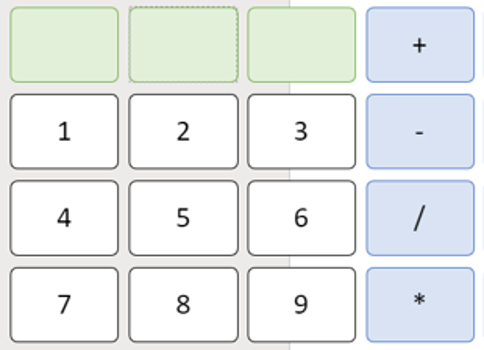
\includegraphics[scale=1]{img/beispiellayout-zum-speichern}
	\caption[Beispiellayout zum Speichern]{Beispiellayout zum Speichern\footnotemark}
\end{figure}
\footnotetext{eigene Darstellung}
\FloatBarrier

Die Kacheln sind in einem vier-mal-vier Format angelegt. Sie bestehen aus drei Stack-Kacheln, neun Operanden-Kacheln, mit einzelnen Zahlen, und vier Operatoren-Kacheln. Diese sind repräsentativ für dieses Beispiel, da der Speicherprozess für alle Inhalte einer Art gleich gehandhabt wird.

Nachfolgend ist die CSV-Repräsentation des obigen Layouts abgebildet. 

\begin{figure}[h]
	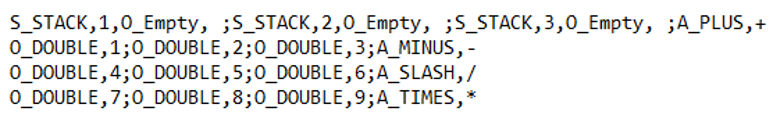
\includegraphics[scale=1]{img/csv-repraesentation-layout}
	\caption[CSV-Repräsentation des Beispiellayouts]{CSV-Repräsentation des Beispiellayouts\footnotemark}
\end{figure}
\footnotetext{eigene Darstellung}
\FloatBarrier

Entsprechend den CSV-Konventionen beschreibt ein Line Break \code{\\n} das Ende einer Reihe des Layouts. Ein Semikolon \code{;} beschreibt das Ende einer Spalte. Innerhalb einer einzelnen Zelle werden die Informationen über eine Kachel durch ein Tupel gehalten. Innerhalb des Tupels werden die einzelnen Werte durch ein Komma \code{,} getrennt.

In der Regel werden pro Kachel zwei Informationen gespeichert: Die Art der Kachel und der Inhalt oder anzuzeigende Text. So beschreibt das Tupel \code{O\_DOUBLE,1} eine Kachel vom Typ \code{ODouble} mit dem Inhalt \code{1}. Lediglich bei \code{Stack}- und \code{HistoryStack}-Kacheln muss ein Tupel mit vier Inhalten gespeichert werden. Der erst Wert beschreibt auch dort die Art der Kachel. Im zweiten Wert wird der Rang des Stacks, also welche Nummer es im Stack hat, gespeichert. Anschließend wird der enthaltene Operand gespeichert. 

\subsubsection{Klasse: TileLayoutManager}
Das Speichern und Laden von CSV-Dateien wird durch diese Klasse implementiert.

\code{loadLayout()}: Laden eines Standardlayouts oder verweis auf den internen Speicher

\code{saveLayout()}: Speichert eine CSV in dem internen Speicher 

\code{wirteLayout()}: Speichert eine CSV in dem internen Speicher 

\code{readLayout()}: Liest eine CSV aus dem internen Speicher ein 

\code{getSavedLayouts()}: Gibt eine Liste der gespeicherten Layouts und Standardlayouts (Für Presenter) 

\code{clearLayouts()}: Löscht alle gespeicherten Layouts (Für Presenter)

\subsubsection{Klasse: TileLayoutFactory}
Die Umformatierung einer CSV-Eingabe in ein \code{TileLayout} wird in dieser Klasse implementiert.

\code{createLayout()}: Orchestriert das einlesen der CSV Datei und der Erstellung des TileLayouts. \\
\code{loadLayout()}: Erstellen des TileLayouts aus der CSV
